\documentclass{article}
\usepackage[utf8]{inputenc}
\usepackage[margin=1in]{geometry}
\usepackage{graphicx}
\usepackage[export]{adjustbox}
\usepackage{amsmath}
\usepackage[ruled,vlined]{algorithm2e}

\title{Machine Learning Overview}
\author{Hanchung Lee}
\date{February 2020}

\begin{document}

\maketitle

\section{Linear Regression}

\noindent
\begin{enumerate}
    \item \textbf{What are the basic concepts? What problem does it solve?}
    \noindent 
    \smallbreak
    Linear Regression, in essence, is trying to fit a hyperplane through the data points that minimizes the sum of the distances of all the points to that hyperplane. That hyperplane is then used to predict the location of new data points. In other words, linear regression is a model $\emph{f} : \mathbb{R}^{d+1} \rightarrow \mathbb{R}$ for a given data pair $(x, y)$ where $x \in \mathbb{R}^{d+1}$ and $y \in \mathbb{R}$. It is if if the function \emph{f} is linear, with weights $w$ of the model is the parameters to be learned. Since regression is a mapping to $\mathbb{R}$, it can be used to estimate a value given a set of inputs $x$.
    
    \item \textbf{What are the assumptions?}
    \noindent 
    \smallbreak
    Regression assumes that the output $y$ is linearly dependent on $x$. However, it will be linear dependent as long as $w$ is linear. It also assumes error term is a normally distributed random variable.
    
    \item \textbf{What are the steps of the algorithm?}
    \noindent 
    \smallbreak
    We model linear regression problem $\mathbf{y} = \mathbf{X}\mathbf{w} + \mathbf{b}$ using both least squares (LS) or maximum likelihood (ML) solutions:
    $$\mathbf{LS}: \; arg \min_{w} \left\|y - \mathbf{X}w\right\|_{2}^{2}$$
    $$\mathbf{ML}: \; arg \max_{w} -\frac{1}{2\sigma}\left\|y - \mathbf{X}w\right\|_{2}^{2}$$
    Or, alternatively, solving it using vector calculus approach, we solve $\frac{\partial}{\partial{X}}\left\|\mathbf{X}\mathbf{W} + \mathbf{b}\right\|_{2}^{2} = 0$, and we get
    $$\mathbf{X} = (\mathbf{W}^T\mathbf{W})^{-1}\mathbf{W}^T\mathbf{b}$$
    
    \item \textbf{What is the cost function?}
    \noindent 
    \smallbreak
    Regression can be done using loss functions that spans the $\mathbb{R}$ space. Mean square error and mean absolute error are the common cost function of choice. We used mean squared error for our formulation.\\
    \smallbreak
    Mean squared error (L2 error)  $\left\|y - y'\right\|_{2}^2 = (y - \mathbf{X}w)^2$ \\ 
    
    \item \textbf{Whare are the advantages/disadvantages?}
    \noindent 
    \smallbreak
    Linear regression is one of the most fundamental machine learning model. It is easy to implement and train. The trained model is also highly explainable. The modeling framework can be extended by different tricks to make it more robust, such as feature engineering/extension/selection, kernel tricks, and adding regularization.
    
    On the flip side, linear regression only model linear relationships between dependent and independent variables (which can be polynomials), which is not enough for more complex relationships. It is also sensitive to anomalies and requires data normalization to prevent that. Also, it requires more samples than the number of parameters as a rule of thumb, which is common across most machine learning models.
    
\end{enumerate}

\section{Ridge Regression}

\noindent
\begin{enumerate}
    \item \textbf{What are the basic concepts? What problem does it solve?}
    \noindent 
    \smallbreak
    Ridge regression is an extension of base regression with an \verb|L2 norm| regularization term $\mathbf{\lambda}\left\| \mathbf{W}\right\|_{2}^{2}$ where $\mathbf{\lambda}$ is the learning rate that adjusts the regularization of parameters $\mathbf{W_{i}}$. \cite{1} The $\mathbf{\lambda}$ term is also called the \emph{shrinkage}. And when $\mathbf{\lambda} = 0$, it is just regular linear regression.
    
    In other words, we use ridge regression to fix if a linear regressor has high variance to improve the out of the sample fit of the model. We can find the learning rate parameter $\lambda$ using cross validation.
    
    \item \textbf{What are the assumptions?}
    \noindent 
    \smallbreak
    As with linear regression, Ridge regression assumes that the output $y$ is linearly dependent on $x$. However, it will be linear dependent as long as $w$ is linear. It also assumes error term is a normally distributed random variable.
    
    \item \textbf{What are the steps of the algorithm?}
    \noindent 
    \smallbreak
    From the descriptions above, we can model ridge regression as linear regression problem with a regularization term.
    $$\mathbf{y} = \mathbf{X}\mathbf{W} + \mathbf{b} + \lambda\left\|\mathbf{W}\right\|_{2}^{2}$$
    Thus, the loss function using least squared solution would be:
    $$\mathbb{L}_{W_{ridge}} = \left\|\mathbf{y} - (mathbf{X}\mathbf{W} + \mathbf{b})\right\|_{2}^{2} + \lambda\left\|mathbf{W}\right\|_{2}^{2}$$
    Pulling in the bias term into W and solving it for \mathbf{W}, we get: 
    $$\mathbf{W} = (\lambda\mathbb{I} + \mathbf{X}^{T}\mathbf{X})^{-1}\mathbf{X}\mathbf{y},$$
    where the $\lambda$ term gets cancelled out as $\lambda$ goes to $\infty$.
    
    \item \textbf{What is the cost function?}
    \noindent 
    \smallbreak
    Regression can be done using loss functions that spans the $\mathbb{R}$ space. Mean square error and mean absolute error are the common cost function of choice. We used mean squared error for our formulation.\\
    \smallbreak
    Mean squared error (L2 error)  $\left\|y - y'\right\|_{2}^2 = (y - \mathbf{X}w)^2$ \\
    \smallbreak
    
    \item \textbf{Whare are the advantages/disadvantages?}
    \noindent 
    \smallbreak
    Ridge regression extends from Linear regression with a regularization term. Thus it shares similar properties as linear regression: easy to implement, easy to train. The trained model is also highly explainable. The modeling framework can be extended by different tricks to make it more robust, such as feature engineering/extension/selection.
    
    On the flip side, it also shares some of the problems with linear regression only model, where it expects linear relationships between dependent and independent variables (which can be polynomials), which is not enough for more complex relationships. It is also sensitive to anomalies and requires data normalization to prevent that. Also, it requires more samples than the number of parameters as a rule of thumb, which is common across most machine learning models.
    
\end{enumerate}

\section{Lasso Regression}

\noindent
\begin{enumerate}
    \item \textbf{What are the basic concepts? What problem does it solve?}
    \noindent 
    \smallbreak
    Lasso regression is an extension of basic regression with an \verb|L1 norm| regularization term $\mathbf{\lambda}\left\| \mathbf{W}\right\|_{1}$ where $\mathbf{\lambda}$ is the learning rate vector that adjusts the regularization of parameters $\mathbf{W_{i}}$. \cite{1} The $\mathbf{\lambda}$ term is also called the \emph{shrinkage}
    
    In other words, Lasso is similar to Ridge where both helps adding biases to the model to improve the out of the sample fit of the model.
    Lasso is especially useful for dealing with sparse data.

    \item \textbf{What are the assumptions?}
    \noindent 
    \smallbreak
    The same as regression, assuming \verb|i.i.d.| of sampled data.
    
    \item \textbf{What are the steps of the algorithm?}
    \noindent 
    \smallbreak
    Same as regression except adding an L1 norm term to penalize Weight coefficients of some variables. 
    
    Cross validation is used to select the regularization hyperparameter $\mathbf{\lambda}$.
    
    \item \textbf{What is the cost function?}
    \noindent 
    \smallbreak
    $$\mathbf{W}^{lasso} = {argmin}_\mathbf{W}} \left\{\frac{1}{2} \sum_{i = 1}^{N} (y_i - \mathbf{W}_0 - \sum_{j=1}^{P} x_{ij}\mathbf{W}_{j})^2 + \mathbf{\lambda}\sum_{j=1}^{P}\left\|\mathbf{W}_{i}\right\|_{1}\right\}$$ \cite{1}, where the first term within the $argmin$ is the mean squared error and the second term is the Lasso regularization. This can be solved with convex optimization.
    
    \item \textbf{Whare are the advantages/disadvantages?}
    \noindent 
    \smallbreak
    The prime difference between Lasso (L1) vs Ridge (L2) regularization of regression is that Lasso has the capability of forcing coefficients to $0$, and in effect, zeros out an feature variable. In essence, Lasso regression is doing feature selection.
    
    In a geometric sense, in high dimeisions, L1 norm will have many sharped edges and corners. During convex optimization, if the optimization hits the edges or corners, the coefficient become zero.  ON the other hand, L2 norm is a smooth surface thus it won't hit exactly model
    
    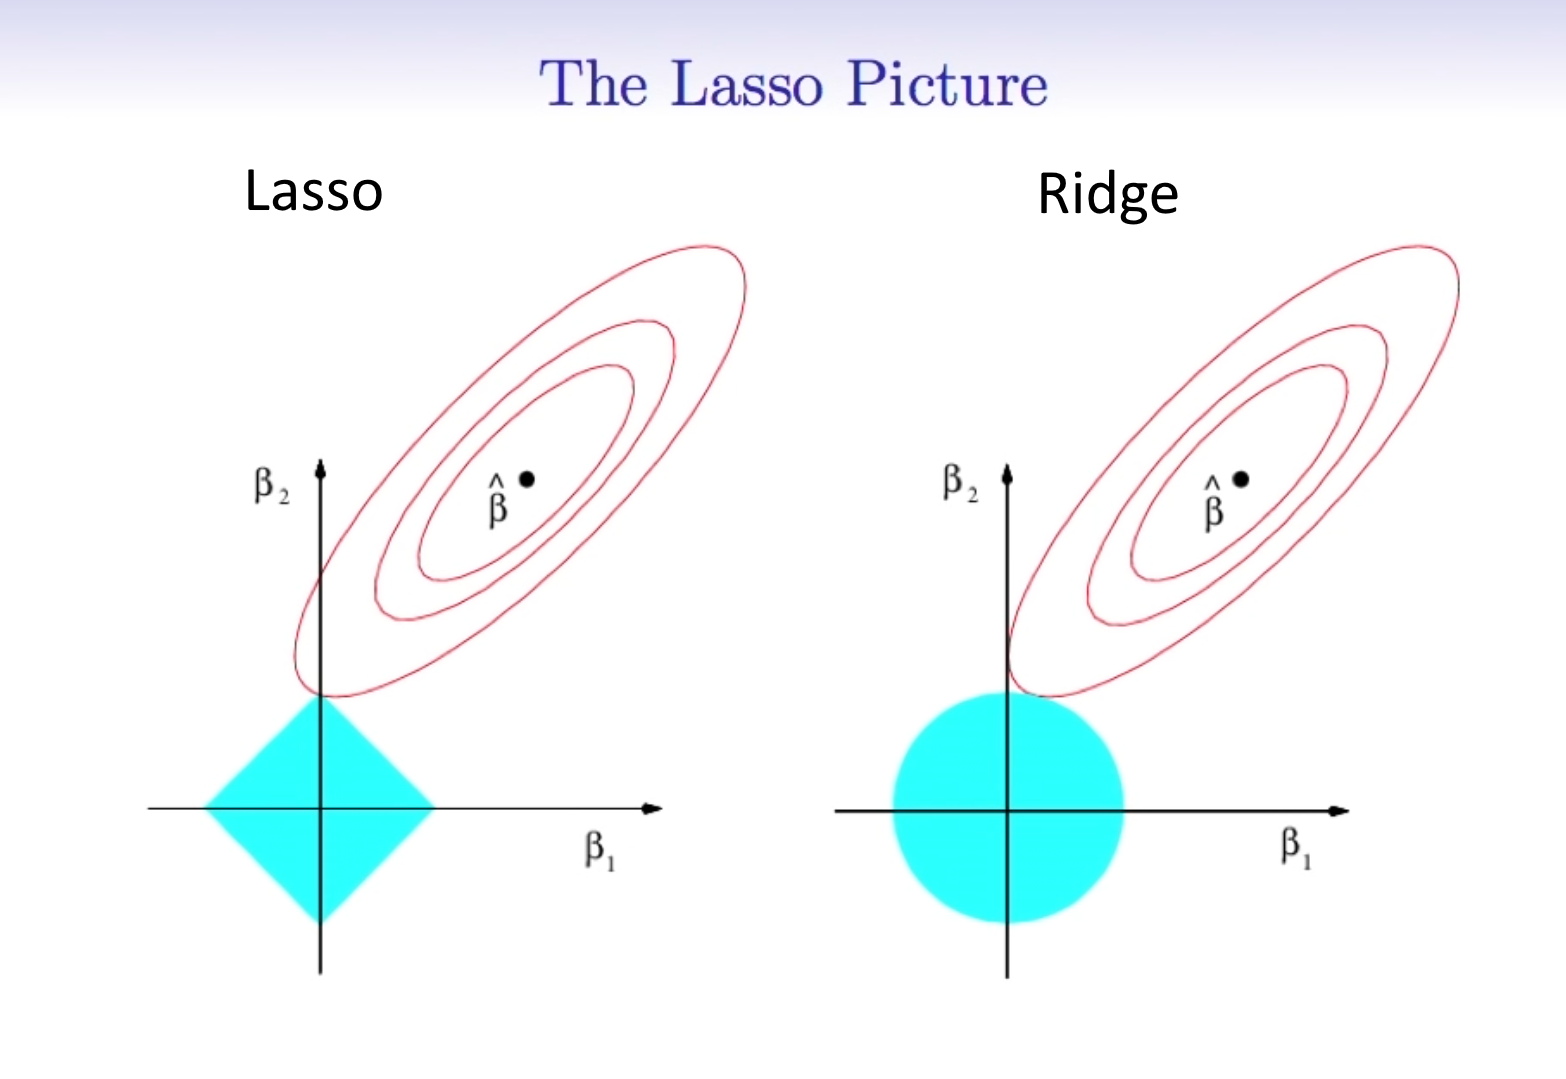
\includegraphics[width=0.5\textwidth, center]{ridge_vs_lasso.png}
    
    Thus, we can say that Lasso Regression yields a \emph{sparse} model where only a subset of the variables is in play. 
    
    Ridge is more suited for models with dense features while Lasso is more suited for models with sparse features. Use cross validation to determine the most suitable regularization.
\end{enumerate}


\bigbreak\bigbreak\bigbreak\bigbreak\bigbreak\bigbreak\bigbreak\bigbreak\bigbreak\bigbreak
\section{Gradient Boosting}
\noindent
\begin{enumerate}
    \item \textbf{What are the basic concepts? What problem does it solve?}
    \noindent 
    \smallbreak
    Gradient boost decision tree models works by training many trees in sequence and ensemble the trees together at the end. When training sequentially, each of the newer trees are trained on the residual error observed by the previous tree. GBDT models tends to fit the training data well, with low bias and high variances. Because of that, it uses a learning rate $\lambda$ to scale contribution from a new tree. The idea is to take many small steps towards the right direction and ensemble them together result in a better prediction.

    \item \textbf{What are the assumptions?}
    \noindent 
    \smallbreak
    Decision tree based models makes no assumption about the distribution of the underlying data. In other words, decision trees are non-parametric.
    
    \item \textbf{What are the steps of the algorithm?}
    \noindent 
    \smallbreak
    Gradient boost initializes by building \verb|depth=1| node. It builds a tree depending on the depth and splits parameters. Then for the following trials it kept on building new trees to minimize the residual errors $(y - \gamma)$from the previous tree, and scale the contribution with a learning rate $\lambda$. The whole process is repeated $M$ times and the maximum depth of the individual trees is $J$.
    
    A formal definition is as follows \cite{1}
    \bigbreak
    \noindent
    \hline
    \textbf{Algorithm} Gradient Tree Boosting Algorithm
    \hline
    \begin{enumerate}
        \item Initialize $f_o(x) = argmin_{\gamma} \sum_{i=1}^{N} L(y_i, \gamma)$
        \item For \emph{m} = 1 to \emph{M}:
            \begin{enumerate}
                
                \item For \emph{i} = 1, 2, . . . , \emph{N} compute the pseudo residual term
                $r_{im} = -\left[ \frac{\partial L(y_i, f(x_i))}{\partial f(x_i)}\right]_{f = f_{m-1}}$
                \item For a regresion tree to the target $\emph{r}_{im}$ given terminal regions $R_{jm}, j = 1, 2, ..., J_m$
                \item For $j = 1, 2, ..., J_m$, find the new predicted value $\gamma$ \\
                $\gamma_{jm} = argmin_{\gamma} \displaystyle\sum_{x_i \in R_{jm}} L(y_i, f_{m-1}(x_i) + \gamma)$
                \item Update $f_m(x) = f_{m-1}(x) + \lambda \sum_{j=1}^{J_m} \gamma_{jm} I(x \in R_{jm})$
            \end{enumerate}
        \item Output $\hat f(x) = f_M(x)$
    \hline
    \end{enumerate}


    
    \item \textbf{What is the cost function?}
    \noindent 
    \smallbreak
    Given the standard loss function setup, $L(f) = \sum_{i=1}^{N} L(y_i, f(x_i))$, proper loss function $L(f)$ can be used for different settings. A summary table is as follows \cite{1}:
    \begin{center}
      \begin{tabular}{ l | l | l }
        \hline
        Setting & Loss Function & $ \frac{-\partial L(y_i, f(x_i))}{\partial f(x_i)}$ \\ \hline
        Regression & $\frac{1}{2}[y_i - f(x_i)]^2$ & $y_i - f(x_i)$ \\ \hline
        Regression & $\left\||y_i - f(x_i)|\right\|$ & sign[y_i - f(x_i)] \\ \hline
        Regression & Huber & y_i - f(x_i) for |y_i - f(x_i)| \leq \delta_m \\ 
         & & \delta_m sign[y_i- f(x_i)] for |y_i - f(x_i)| > \delta_m \\ 
         & & where \delta_m \eq \alpha th-quantile \{|y_i - f(x_i)|\} \\ \hline
        Classification & Multinominal Deviance & \emph{k}th component: $I(y_i \eq G_k) - p_k(x_i)$ \\
        \hline
      \end{tabular}
    \end{center}
    
    \item \textbf{What are the advantages/disadvantages?}
    \noindent 
    \smallbreak
    Gradient boost is very similar to AdaBoost. The key difference is that for Gradient Boost, it can have a tree size that is larger than a stomp (depth of 1). Because gradient boosting is a boosting model that ensembles sequentially trained models, it is a naturally a low bias model. However, the downside is to a low bias model is the variance can be high and has to be reduced by adding regularization. Also, because the model is trained sequentially, it is compute intensive to train.
    
\end{enumerate}


\section{K-Nearest Neighbors}
\noindent
\begin{enumerate}
    \item \textbf{What are the basic concepts? What problem does it solve?}
    \noindent 
    \smallbreak
    K-Nearest Neighbors can be used for either regression or classification. It finds the K nearest points next to a new input data and determines the value or class by taking the mean value of its K nearest neighbors, or in the case of classification, mode. It captures the point similarity with its neighbours.
    
    The smaller the K, smaller training error; the larger the K, the more smooth the decision boundary due to majority voting of neighbors. To find the optimal K, cross validate or grid search.

    \item \textbf{What are the assumptions?}
    \noindent 
    \smallbreak
    KNN is a non parametric model. The basic assumption is that the data points close to it will have the same class labels for classification, or similar values in terms of regression.
    
    \item \textbf{What are the steps of the algorithm?}
    \noindent 
    \smallbreak
    Given data $(x_1, y_1), (x_2, y_2), ..., (x_i, y_i)$, construct KNN as follows:
    For a new input $x$:
    \begin{enumerate}
        \item Return $k$ nearest points closest to $x$, indexed as $x_{i1}, x_{i2}, ..., x_{ij}$.
        \item Return the majority vote of $y_{i1}, y_{i2}, ..., y_{ij}$.
    \end{enumerate}
    
    \item \textbf{What is the cost function?}
    \noindent 
    \smallbreak
    KNN does not use a loss function to train the model. Instead, it uses distance functions, where the most common distance function is \verb|L2 norm| $= \left\|u - v\right\|_2 = (\sum_{i=1}^{d}(u_i - v_i)^{2})^\frac{1}{2}$ for dimension $\mathbb{R}^d$. Or, in a more generalized form,\\
    $$\left\|u - v\right\|_p = (\sum_{i=1}^{d}(u_i - v_i)^{p})^\frac{1}{p}$$
    
    Other distances can be used as well, including edit distances (how many edits away to transform from one string to another), or correlation distance (for signal detection).
    
    \item \textbf{What are the advantages/disadvantages?}
    \noindent 
    \smallbreak
    KNN has an easy to interpret output and it does not make any assumption about the underlying data. Further, it can naturally extend to multi-class classifier and can do well in practice with enough data. For example, KNN can achieve 90\%+ with MNIST dataset.
    
    Om the other hand, it requires data to in or relatively close to memory, thus when the dataset is big is big enough it becomes a big search problem. Also, finding a proper distance function requires some expert knowledge, heuristics, or a grid search.
\end{enumerate}
\bigbreak\bigbreak\bigbreak\bigbreak\bigbreak\bigbreak\bigbreak\bigbreak\bigbreak\bigbreak


\section{K-means Clustering}
\noindent
\begin{enumerate}
    \item \textbf{What are the basic concepts? What problem does it solve?}
    \noindent 
    \smallbreak
    K-means is an unsupervised learning method where it tries to separate data into $K$ clusters by finding the $K$ centroids within the dataset.
    
    \item \textbf{What are the assumptions?}
    \noindent 
    \smallbreak
    K-means is a non-parametric unsupervised learning model. It assumes the clusters separated/calculated has a "circular" shape with a centroid each  as it attempts to assign each sample $(x_1, ..., x_n)$ to one of the $K$ clusters $\{C_1, ..., C_k\}$
    
    \item \textbf{What are the steps of the algorithm?}
    \noindent 
    \smallbreak
    To run K-means clustering, we use the following algorithm:
    
    \begin{algorithm}
        Initialize randomly centeroids $\mu_1, ..., \mu_k$\;
        \Repeat{convergence}{
            assign each point $x_i$ to the cluster with the closet $\mu_j$;\\
            Calculate the new mean for each cluster as follows:;\\
            $\mu_j = \frac{1}{\|C_j\|} \sum_{x_i \in C_j} x_i$\\}
        \caption{K-means algorithms}
        Convergence: means no change in the clusters OR maximum number of iterations reached.
    \end{algorithm}
    
    To find the optimal $k$ that clusters the data, we can use PG-means algorithm \cite{5}. Other alternatives are G-means and P-means.
    \begin{algorithm}
        Initialize $k$ to be a small number;
        \Repeat{no more cluster center is created.}{
            Run K-means with those cluster centers, and store the resulting center as C\\
            Assign each point to its nearest cluster\\
            Determine if points in each cluster fit a Gaussian distribution (using Anderson-Darling test).\\
            For each cluster, if the points seem to be normally distributed, keep the cluster center. Otherwise replace it with two cluster centers.}
        \caption{PG-means algorithm}
    \end{algorithm}
    
    \item \textbf{What is the cost function?}
    \noindent 
    \smallbreak
    There's no cost functions for K-means clustering per se, but the algorithm uses $\mu_j = \frac{1}{\|C_j\|} \sum_{x_i \in C_j} x_i$ to calculate the mean of each centroid.
    
    \item \textbf{What are the advantages/disadvantages?}
    \noindent 
    \smallbreak
    The biggest benefit for K-means Clustering as a clustering algorithm is that its super easy to implement.
    
    However there are many downsides. First, it needs to know $K$, which we can 'solve' using PG-means algorithm\cite{5}, but there still exists no trivial way to evaluate the model similar to, say, comparing to counting the number of errors in a classification. K-means also suffers from the curse of dimensionality and has no theoretical foundation.
    
    There are other methods to cluster non-circular shapes, such as spectral clustering, DBScan, BIRCH, etc that handles other shapes. Alternatively, we can use PCA and TSNE for clustering higher dimensional data.
\end{enumerate}



\section{Naive Bayes}

\noindent
\begin{enumerate}
    \item \textbf{What are the basic concepts? What problem does it solve?}
    \noindent 
    \smallbreak
    Naive Bayes classifier is a probabilistic model based on the Bayes rule. It is Naive because it makes an assumption that inputs are conditionally independent of each output class, which is not realistic. It is also known as "Idiot's Bayes"\cite{1}. Despite that, naive Bayes classifiers often outperform far more sophisticated alternatives. It's a simple and strong method that can be comparable to decision trees and neural networks in certain cases.
    
    It is most commonly seen and used in text classification models. 
    
    \item \textbf{What are the assumptions?}
    \noindent 
    \smallbreak
    
    It is Naive because it makes an assumption that inputs are conditionally independent of each output class, which is not realistic. It is also known as "Idiot's Bayes"\cite{1}.
    
    \item \textbf{What are the steps of the algorithm?}
    \noindent 
    \smallbreak
    \textbf{Learning:} Based on the frequency counts in the dataset:
    \begin{enumerate}
        \item Estimate all $p(y), \forall y \in \mathbb{Y}$
        \item Estimate all $p(x_i|y), \forall y \in \mathbb{Y}, \forall x_i$
    \end{enumerate}
    \textbf{Classification:} For a new example, use:\\
    \begin{align*}
        y_{new} = argmax_{y \in \mathbb{Y}} \mathbf{\Pi}_{i} p(x_i|y)    
    \end{align*}
    
    No model per se or hyperplane, just count the frequencies of various data combinations within the training examples.
    
    \item \textbf{What is the cost function?}
    \noindent 
    \smallbreak
    "Cost" function for naive Bayes is not the same as algorithms, where other algorithms try to adjust the model weights with regards to the value that the cost function outputs. Naive Bayes is simply doing 
    \begin{align*}
        y_{new} = argmax_{y \in \mathbb{Y}} \mathbf{\Pi}_{i} p(x_i|y)    
    \end{align*}
    
    \item \textbf{Whare are the advantages/disadvantages?}
    \noindent 
    \smallbreak
    Naive Bayes is a linear classifier, an variant of Linear Discrimanent Analysis. It is incredibly simple and easy to implement and works wonderfully for text data. It is especially appropriate when the dimension of the feature space is high. The model is light weight and runs very fast for real time inferencing. It is especially useful when inference time budget is small.
    
    The naive assumption of feature Independence is a double edged sword. While the assumption made naive Bayes a simple and powerful model, the assumption also prevent it to learn further intricacies of the underlying relationships. One other major disadvantage of naive Bayes is that it does not generalize well to unseen inputs.
    
\end{enumerate}
\pagebreak

\section{Support Vector Machines}
\noindent
\begin{enumerate}
    \item \textbf{What are the basic concepts? What problem does it solve?}
    \noindent 
    \smallbreak
    Support Vector Machines finds the hyperplane that separates the data with the greatest margin. Two key concepts of Support Vector Machine is it uses soft margins instead of max margins to reduce variances and it uses the kernel trick to implicitly increase the feature space to reduce bias. 
    
    It can be used for both classification and regression problems. It uses a kernel function to compute the inner product of two variables in a higher dimensional space. The data that resides in the soft margin are called support vectors, with distance to the soft margin line $\epsilon$. Hyperparameter \textbf{C} is learning rate and is found using cross validation.
    
    \item \textbf{What are the assumptions?}
    \noindent 
    \smallbreak
    Support Vector Machine treats all the data points as equals so it is important to standardize the data. Otherwise it does not make assumptions about the underlying data distribution.
    
    \item \textbf{What are the steps of the algorithm?}
    \noindent 
    \smallbreak
    Support Vector Machine is a convex optimization problem where it \textbf{Solve:} $\min_{w, b, \epsilon}\frac{1}{2}\left\|w\right\|_{2}^{2} + C\sum_{i=1}^{n} \epsilon_i$ such that $y_i(w^{T} x_i - w_0) \geq (1 - \epsilon_i)$ and $\epsilon_i \geq 0, \quad \forall i$. After derivation, Support Vector Machine function is:
    $$f(x) = w_o + \sum \hat{\alpha_i}K(x, x_i)$$
    where $\hat{\alpha_i}$ are zero for data not in the support set and $K$ is the Kernel function. The common kernels are polynomial, radio basis kernel (behaves similar to nearest neighbor), and neural network kernel. \cite{1}
    \begin{center}
      \begin{tabular}{ l l }
        \hline
        nth-Degree polynomial & $K(x,x') = (1 + (x, x'))^d$ \\
        Radial basis function (RBF) & $K(x, x') = exp(-\gamma\left\|x - x'\right\|_{2}^{2}$ \\ 
        Neural network & $K(x, x') = tanh(\kappa_1(x, x') + \kappa_2)$ \\ 
        \hline
      \end{tabular}
    \end{center}
    
    \item \textbf{What is the cost function?}
    \noindent 
    \smallbreak
    Support Vector Machine uses hinge loss, which has the form of loss plus penalty. $L[y, f(x)] = [1 - yf(x)]_{+}$The following compares the negative log likelihood loss to hinge loss. Note that sharp hinge corner, that is when $\aplha$ are set to zero.
    
    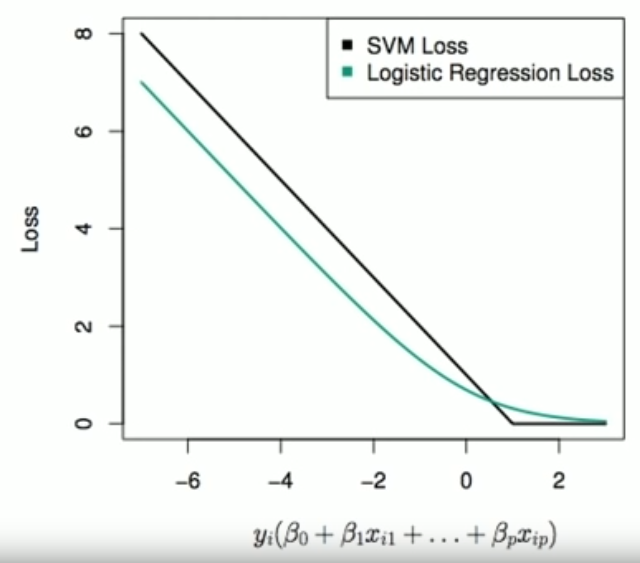
\includegraphics[width=0.3\textwidth, center]{hinge_loss_han.png}
    
    \item \textbf{Whare are the advantages/disadvantages?}
    \noindent 
    \smallbreak
    When classes are nearly separable, SVM does better than logistic regression and LDA. When classes are not, then SVM does similarly well as logistic regression. We can use kernel tricks with LDA and logistic regression as well, but more compute intensive.
    
    The downside with SVM is it does not provide a probability estimate, low interpretability, and does not do any feature selection.
    
\end{enumerate}


\section{Neural Networks}
\noindent
\begin{enumerate}
    \item \textbf{What are the basic concepts? What problem does it solve?}
    \noindent 
    \smallbreak
    According to the Universal Approximator Theorum, neural networks is an universal function approximator that can be used approximate any functions that map $X \rightarrow Y$. It can be used abstracts away some of the feature engineering steps in classical machine learning tasks. For example, instead of designing image filters, CNN learns the filters itself, or instead of tagging word semantic labels, RNNs learns the relationships between words.
    
    The most fundamental neural network layer is a linear layer where $f(\mathbf{X}) = \sum_{m=1}^{M} g_m(\mathbf{W_m}\intercal\mathbf{X})$, where the input values go through an affine transformation and scaled by an activation function $g_m$. Activation functions usually tend to scale the outputs to pseudo range bound, such as Sigmoid and Tanh. 

    \item \textbf{What are the assumptions?}
    \noindent 
    \smallbreak
    The assumptions are highly dependent on the structure of neural networks. For example, some neural network architectures such as convolution neural networks or recurrent neural nets assumes that the underlying data are \emph{i.i.d} while some other architectures such as Bayesian neural networks or Graph neural nets could have different assumptions about the relationships between feature spaces.
    
    \item \textbf{What are the steps of the algorithm?}
    \noindent 
    \smallbreak
    Neural networks is predominant solved using stochastic gradient descent with an auto differentiation library. First, inputs are feed forward through the network for an output $\hat y$, and apply the loss function. The algorithm then take the gradients of the loss function and back propagate the network to obtain the differences in parameters between target and output. The parameters are then updated with the differences. One small batch at a time.
    \bigbreak
    \hline
    \noindent
    \textbf{Algorithm} Stochastic gradient descent (SGD) update at training iteration k \cite{2}
    \hline
    \smallbreak
    \textbf{Require:} Learning rate $\epsilon_k$
    
    \textbf{Require:} Initial parameter $\theta$
    
    \qquad \textbf{while} stopping criterion not met \textbf{do}
    
    \qquad \qquad Sample a minibatch of \emph{m} examples from the training set $\{x^{(1)}, ..., x^{(m)}\}$ with corresponding targets $y^{(i)}$
    
    \qquad \qquad Compute gradent estimate: $\hat g \leftarrow + \frac{1}{m}\nabla_{\theta}\sum_{i} L(f(x^{i};\theta),y_{(i)})$
    
    \qquad \qquad Apply update: $\theta \leftarrow \theta - \epsisolon\hat g$
    
    \qquad \textbf{end while}
    \smallbreak
    \hline

    \item \textbf{What is the cost function?}
    \noindent 
    \smallbreak
    Neural networks is an flexible architecture thus different loss functions can be used for different tasks. Typical loss functions includes cross entropy and negative log likelihood for classification and mean absolute error (L1) and mean squared error (L2) for regressions.
    
    \item \textbf{Whare are the advantages/disadvantages?}
    \noindent 
    \smallbreak
    Rather than considering neural networks as a kind of model, it is closer to a highly customizable building blocks for machine learning models. Depends on the complexity of the network constructed, it can be capable of learning a large amount of information from data. At the same time it excels in learning implicit relationships. 
    
    However, it is an black box model that is quite difficult to interpret and usually has to rely on large data sets and large amount of compute power to train. It is also difficult to debug and fine tune.
    
\end{enumerate}


\section{Generative vs Discriminative}
\noindent
\begin{enumerate}
    \item \textbf{What are the basic concepts?}
    \noindent 
    \smallbreak
    \textbf{Generative classifiers} learns a model of the join probability $p(x, y)$, of the input $x$ and the label $y$, and make their predictions by using Bayes rules to calculate $p(y|x)$, then pick the most likely label $y$.\cite{4} In learning joint probability $p(x, y)$ it learns both $p(x|y)$ (likelihood) and $p(y)$ (class prior) and make inference using Bayes rule. Generative models can use the joint probability $p(x, y)$ to generate new data similar to existing data. It also requires not as much data samples to train and easy to implement.
    \begin{itemize}
        \item[--] Idea: Build a model for what positive examples look like. Build a different model for what negative example look like.
        \item[--] To predict a new example, match it with each of the models and see which match is best.
        \item[--] Model $p(x|y)$ and $p(y)$
        \item[--] Use Bayes rule to obtain $p(y|x) = \frac{p(x|y)p(y)}{p(x)}$
        \item[--] To make a prediction: \\
        \begin{align*}
            argmax_{y} p(y|x) &= argmax_{y} \frac{p(x|y)p(y)}{p(x)} \\
              &\approx argmax_{y} p(x|y)p(y)  \\ 
        \end{align*}
        
    \end{itemize}

    \noindent 
    \smallbreak
    \textbf{Discriminative classifiers} models the posterior $p(y|x)$ directly, or learn a direct map from input $x$ to class labels.\cite{4} Discriminative models generally offers better performance in classification tasks.
    \begin{itemize}
        \item[--] Idea: model $p(y|x)$, conditional distribution of $y$ given $x$.
        \item[--] In discriminative algorithms: find a decision boundary that separates positive from negative examples
        \item[--] To predict a new example, check which side of the decision boundary it falls
        \item[--] Model $p(y|x)$ directly.
    \end{itemize}
    
    \noindent 
    \smallbreak
    Here are some examples of generative and discriminative models:
    \begin{center}
      \begin{tabular}{ l l }
        \hline
        \textbf{Generative} & \textbf{Discriminative} \\
        \hline
        Naive Bayes & Logistic regression \\
        Hidden Markov model & K-nearest neighbors \\ 
        Gaussian mixture model & Support vector machines \\
        Generative adversarial networks & Neural networks \\ 
        \hline
      \end{tabular}
    \end{center}
    
\end{enumerate}
\pagebreak

\section{Bias-Variance Trade off}
\noindent
\begin{enumerate}
    \item \textbf{What are the basic concepts?}
    \noindent 
    \smallbreak
    
\end{enumerate}


\begin{thebibliography}{}
\bibitem{1}
Hastie, Tibshirani, and Friedman,
\emph{The Elements of Statistical Learning}.
2nd Edition,
2009.

\bibitem{2}
Goodfellow, Bengio, Courville,
\emph{Deep Learning},
2016

\bibitem{3}
Nasirany, Thomas, Wei, and Yang,
\emph{A Comprehensive Guide to Machine Learning},
2018

\bibitem{4}
Ng and Jordan,
\emph{On Discriminative vs Generative Classifiers: A comparison of logistic regression and naive Bayes}
2002

\bibitem{5}
Hamerly and Elkan
\emph{PG-means: learning the number of clusters in data}
2003

\end{thebibliography}
\end{document}

